\documentclass{beamer}
\usepackage{graphicx}
\usepackage{hyperref}
\usepackage{amsmath}
\usepackage{subfig}
\usepackage{listings}
\usepackage{tcolorbox,fancyvrb,xcolor,tikz}
\tcbuselibrary{skins,breakable}

\newenvironment{VerbatimIN}
 {\VerbatimEnvironment
  \begin{tcolorbox}[
    breakable,
    colback=lightgray,
    spartan
  ]%
  \begin{Verbatim}}
 {\end{Verbatim}\end{tcolorbox}}

 \newenvironment{VerbatimOUT}
 {\VerbatimEnvironment
  \begin{tcolorbox}[
    breakable,
    spartan
  ]%
  \begin{Verbatim}}
 {\end{Verbatim}\end{tcolorbox}}


\title{Mixed Effects Models - Day 4}
\subtitle{Generalised Least Squares - GLS}
\author{Marieke Wesselkamp\\Department of Biometry and Environmental Systems Analysis\\Albert-Ludwigs-University of Freiburg (Germany)}
\date{February 2023}

\begin{document}

\begin{frame}
  \titlepage
\end{frame}

\begin{frame}{Ways to Avoid Mixed Effects Models}
  \begin{itemize}
    \Large 
    \item Ignore dependencies: simply \textbf{wrong}
    \item Take means within groups
    \item Use grouping variable as a covariate
  \end{itemize}
\end{frame}

\begin{frame}[fragile]
\frametitle{Taking Means Within Groups...}
\begin{columns}
    \begin{column}{0.45\textwidth}
        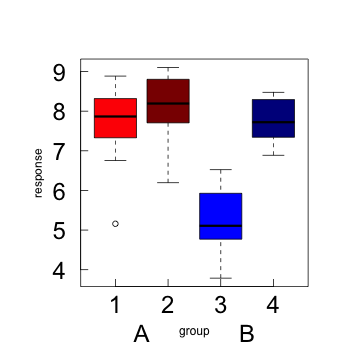
\includegraphics[width=\textwidth]{lectures/day_4_GLS/figures/unnamed-chunk-3-1.png}
    \end{column}
    \begin{column}{0.55\textwidth}
    \tiny
    \begin{VerbatimIN}[numbers=left,numbersep=6pt]
means <- 
data.frame(treat = c(rep("A",2),rep("B",2)), 
           response = c(tapply(response,
                        group, mean)))

summary(aov(response ~ treat, means))        
    \end{VerbatimIN}
    \begin{VerbatimOUT}[numbers=left,numbersep=6pt]
            Df Sum Sq Mean Sq F value Pr(>F)
treat        1  1.766   1.766   1.147  0.396
Residuals    2  3.079   1.539           
    \end{VerbatimOUT}    
      \end{column}
      \end{columns}
      \vspace{0.5cm}

      \textbf{Reduction of 40 data points to 4}
\end{frame}

\begin{frame}[fragile]
    \frametitle{...provides less information and power than accounting for random effects}
    \centering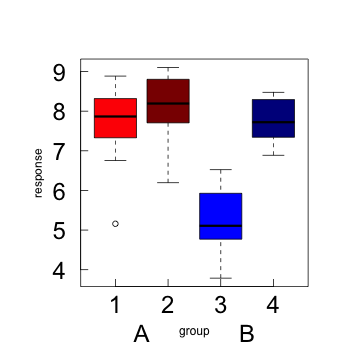
\includegraphics[width=0.4\textwidth]{lectures/day_4_GLS/figures/unnamed-chunk-5-1.png}

    \scriptsize
    \begin{VerbatimOUT}[numbers=left,numbersep=6pt]
Data: NULL
Models:
mod.2b: response ~ 1 + (1 | group)
mod.2a: response ~ treat + (1 | group)
       npar    AIC    BIC  logLik deviance  Chisq Df Pr(>Chisq)
mod.2b    3 119.92 124.98 -56.958   113.92                     
mod.2a    4 120.10 126.86 -56.051   112.10 1.8135  1     0.1781
    \end{VerbatimOUT}

\end{frame}

\begin{frame}[fragile]
  \frametitle{Using grouping as a fixed covariate...}
  \begin{columns}
      \begin{column}{0.4\textwidth}
          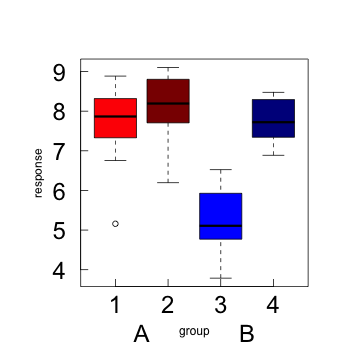
\includegraphics[width=\textwidth]{lectures/day_4_GLS/figures/unnamed-chunk-7-1.png}
      \end{column}
      \begin{column}{0.6\textwidth}
      \tiny
        \begin{VerbatimIN}[numbers=left,numbersep=6pt]
summary(aov(response ~ treat + group))            
        \end{VerbatimIN}

        \begin{VerbatimOUT}[numbers=left,numbersep=6pt]
            Df Sum Sq Mean Sq F value   Pr(>F)    
treat        1  17.66  17.660   23.04 2.76e-05 ***
group        2  30.79  15.394   20.09 1.38e-06 ***
Residuals   36  27.59   0.766                     
---
Signif. codes:  0 '***' 0.001 '**' 0.01 '*' 0.05 
'.' 0.1 ' ' 1            
        \end{VerbatimOUT}
      \end{column}
  \end{columns}
\end{frame}

\begin{frame}[fragile]
    \frametitle{...uses too many degrees of freedom}

    \begin{columns}
        \begin{column}{0.38\textwidth}
            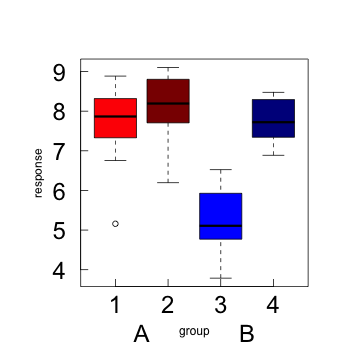
\includegraphics[width=\textwidth]{lectures/day_4_GLS/figures/unnamed-chunk-10-1.png}
        \end{column}
        \begin{column}{0.62\textwidth}
        \tiny
        \begin{VerbatimIN}
summary(lm(response ~ treat + group))            
        \end{VerbatimIN}
        \begin{VerbatimOUT}
Call:
lm(formula = response ~ treat + group)

Residuals:
    Min      1Q  Median      3Q     Max 
-2.4635 -0.3552  0.1093  0.6364  1.2629 

Coefficients: (1 not defined because of singularities)
            Estimate Std. Error t value Pr(>|t|)    
(Intercept)   7.6224     0.2768  27.533  < 2e-16 ***
treatB        0.1070     0.3915   0.273    0.786    
group2        0.4276     0.3915   1.092    0.282    
group3       -2.4443     0.3915  -6.243 3.29e-07 ***
group4            NA         NA      NA       NA    
---
Signif. codes:  0 '***' 0.001 '**' 0.01 '*' 0.05 
'.' 0.1 ' ' 1

Residual standard error: 0.8755 on 
36 degrees of freedom
Multiple R-squared:  0.6371,    
Adjusted R-squared:  0.6069 
F-statistic: 21.07 on 3 and 36 DF,  p-value: 4.708e-08
        \end{VerbatimOUT}

        \end{column}
    \end{columns}
\end{frame}

\begin{frame}{Summary}
1. Taking Means Within Groups provides less information and power than accounting for random effects\\
2. Using grouping as a fixed covariate uses too many degrees of freedom \\
\vspace{0.5cm}

\large\textbf{All these Mixed Effects Models avoidance mechanisms have issues}
\vspace{0.5cm}

  \begin{quote}
    Generalised Least Squares can be a solution.
  \end{quote}
\end{frame}

\begin{frame}{The Linear Model}
  Remember the Linear Model:
  \[
  \mathbf{y} = \mathbf{X} \cdot \mathbf{b} + \mathbf{e}, \quad \epsilon \sim \mathcal{N}(0, \sigma^2_{e} \cdot \mathbf{I})
  \]
  And the residual variance-covariance matrix in a linear model:
  \[
  \mathbf{V} = \sigma^2 \cdot \mathbf{I} = 
  \begin{bmatrix}
  \sigma^2 & 0 & \cdots & 0 \\
  0 & \sigma^2 & \cdots & 0 \\
  \vdots & \vdots & \ddots & \vdots \\
  0 & 0 & \cdots & \sigma^2
  \end{bmatrix}
  \]
\end{frame}

\begin{frame}{Covariance Matrix}
  \centering
  The off-diagonals tell the covariance $covar_{ij}$ between $y_i$ and $y_j$:
  \vspace{0.5cm}

  \[
  \mathbf{V} = 
  \begin{bmatrix}
  \sigma^2 & 0 & \cdots & 0 \\
  0 & \sigma^2 & \cdots & 0 \\
  \vdots & \vdots & \ddots & \vdots \\
  0 & 0 & \cdots & \sigma^2
  \end{bmatrix}
  \]
  \vspace{0.5cm}
  
  Which are defined in a Linear Model as $0$ for \textit{independent} data.
\end{frame}

\begin{frame}{}
  Generalised least squares (GLS) estimation allows to \textbf{explicitly} work with the variance-covariance matrix $\mathbf{V_i}$ of the residuals within a group.
  \vspace{0.5cm}
  
  It let's you define the structure of $\mathbf{V_i}$ and estimate the values in there.
  \vspace{0.5cm}
  
  \begin{itemize}
    \item Different $\sigma^2$ on the diagonals to account for heteroscedasticity
    \item Off-diagonals for non-independency
  \end{itemize}
  \vspace{0.5cm}
  
  \begin{quote}
    This means errors are not $iid$ distributed anymore.
  \end{quote}
\end{frame}

% \begin{frame}[fragile]{R Code Setup for GLS}
%   \begin{verbatim}
% repeated <- read.table("repeated.txt", header = TRUE)
% repmeasures <- read.table("repmeasures.txt", header = TRUE)
% farms <- read.table("farms.txt", header = TRUE)
% farms$farm <- factor(farms$farm)
% fertilizer <- read.table("fertilizer.txt", header = TRUE)
% blowfly <- read.table("blowfly.txt", header = TRUE)
% blowfly$flies <- as.numeric(blowfly$flies)
% blowfly$week <- c(1:362)
% blowfly <- na.omit(blowfly)
% library(lattice)
% library(nlme)
%   \end{verbatim}
% \end{frame}

\begin{frame}{Marginal Model}
  This gives us the Marginal Model:
  \[
  \mathbf{y} = \mathbf{X} \cdot \mathbf{b} + \mathbf{e}, \quad \epsilon \sim \mathcal{N}(0, \mathbf{V_i})
  \]
  The \textbf{marginal model} describes the deterministic part for the average trend in the data while considering the correlation between non-independent data within a group.
\end{frame}

\begin{frame}{Properties of Marginal Model}
  \begin{itemize}
    \item In the Marginal Model fitted with GLS, there are \textbf{NO} random effects.
    \item The Marginal Model ignores the random structure due to grouping and fits directly to the deterministic trend.
  \end{itemize}
  \vspace{0.5cm}
  
  \begin{quote}
    You won't get among- or within-group variances or group-specific (random) intercepts and slopes.
  \end{quote}
\end{frame}

\begin{frame}{Specifying the Covariance Matrix}
  All that matters is in the a-priori specified residual variance-covariance matrix.
  We will continue working with the assumption of homoscedasticity (identically distributed residual variances $\sigma^2$) but will work with different error structures on the off-diagonals.
  \vspace{0.5cm}
  
  \[
  \mathbf{V_i} = 
  \begin{bmatrix}
  \sigma^2 & c_{12} & c_{13} & c_{14} & c_{15} \\
  c_{21} & \sigma^2 & c_{22} & c_{23} & c_{24} \\
  c_{31} & c_{32} & \sigma^2 & c_{34} & c_{35} \\
  c_{41} & c_{42} & c_{43} & \sigma^2 & c_{45} \\
  c_{51} & c_{52} & c_{53} & c_{54} & \sigma^2
  \end{bmatrix}
  \]
\end{frame}

\begin{frame}{Correlation Matrix in GLS}
  In practice, GLS works with the correlation instead of the variance-covariance matrix.
  \[
  \text{cor}(y_i,y_j) = \frac{\text{cov}(y_i, y_j)}{\sqrt{\text{var}(y_i)} \cdot \sqrt{\text{var}(y_j)}}
  \]
  This makes the variance-covariance matrix a correlation matrix:
  \[
  \mathbf{V_i} = 
  \begin{bmatrix}
  1 & \rho_{12} & \rho_{13} & \rho_{14} & \rho_{15} \\
  \rho_{21} & 1 & \rho_{23} & \rho_{24} & \rho_{25} \\
  \rho_{31} & \rho_{32} & 1 & \rho_{34} & \rho_{35} \\
  \rho_{41} & \rho_{42} & \rho_{43} & 1 & \rho_{45} \\
  \rho_{51} & \rho_{52} & \rho_{53} & \rho_{54} & 1
  \end{bmatrix}
  \]
  \vspace{0.5cm}

  \centering \tiny There are many ways to specify $\mathbf{V_i}$; some are built in, but you can write your own and implement it
\end{frame}

\begin{frame}
  \large
  \textbf{Types of Variance Structures}
  \begin{itemize}
    \item General structure
    \item Compound symmetry
    \item Temporal or spatial autocorrelation structures
  \end{itemize}
\end{frame}

\begin{frame}{General Structure}
  Each element above (below) the diagonal has to be estimated: here 10 values.
  \[
  \mathbf{V_i} = 
  \begin{bmatrix}
  1 & \rho_{12} & \rho_{13} & \rho_{14} & \rho_{15} \\
  \rho_{21} & 1 & \rho_{22} & \rho_{23} & \rho_{24} \\
  \rho_{31} & \rho_{32} & 1 & \rho_{34} & \rho_{35} \\
  \rho_{41} & \rho_{42} & \rho_{43} & 1 & \rho_{45} \\
  \rho_{51} & \rho_{52} & \rho_{53} & \rho_{54} & 1
  \end{bmatrix}
  \]
  But with just one more measurement, it would already be 15 values.
  \vspace{0.5cm}
  
  \begin{quote}
    The general structure of $\mathbf{V_i}$ is flexible but data hungry!
  \end{quote}
\end{frame}

\begin{frame}{Compound Symmetry}
  \centering There is only one element to be estimated.
  \[
  \mathbf{V_i} = 
  \begin{bmatrix}
  1 & \rho & \rho & \rho & \rho \\
  \rho & 1 & \rho & \rho & \rho \\
  \rho & \rho & 1 & \rho & \rho \\
  \rho & \rho & \rho & 1 & \rho \\
  \rho & \rho & \rho & \rho & 1
  \end{bmatrix}
  \]
  \vspace{0.5cm}
  
  \begin{quote}
    A compound symmetric $\mathbf{V_i}$ is the simplest form...but also sometimes the least appropriate form.
  \end{quote}
\end{frame}

\begin{frame}{Compound Symmetry - Suitability}
\begin{columns}
    \begin{column}{0.5\textwidth}
    The compound symmetry structure is suitable for cases where repeated measurements are \textbf{not ordered} in time or space, i.e., each value in a group is \textbf{equally} correlated with each other value. In other words, there is no temporal or spatial distance between them. 
    \end{column}
    \begin{column}{0.5\textwidth}
    \centering
    For example, in the \textit{Bloodworm} feeding experiment:
    \vspace{0.5cm}
    
    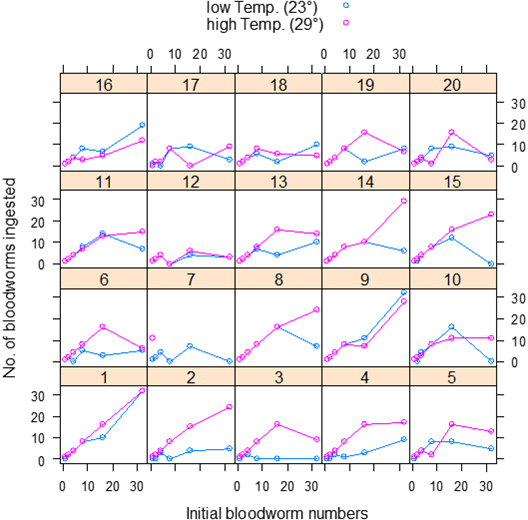
\includegraphics[width=\textwidth]{lectures/day_4_GLS/figures/bloodworms.png}
    \end{column}
\end{columns}
\end{frame}

\begin{frame}{Temporal Autocorrelation}
\begin{columns}
    \begin{column}{0.5\textwidth}
    Temporal autocorrelation matters in experiments like this where similarity between data points is not experimentally broken up but is actually carrying biological information, e.g., about the time-lag of density dependence. 
    \end{column}
    \begin{column}{0.5\textwidth}
    \centering
    For example, in the \textit{Mites} population experiment:
    \vspace{0.5cm}
    
    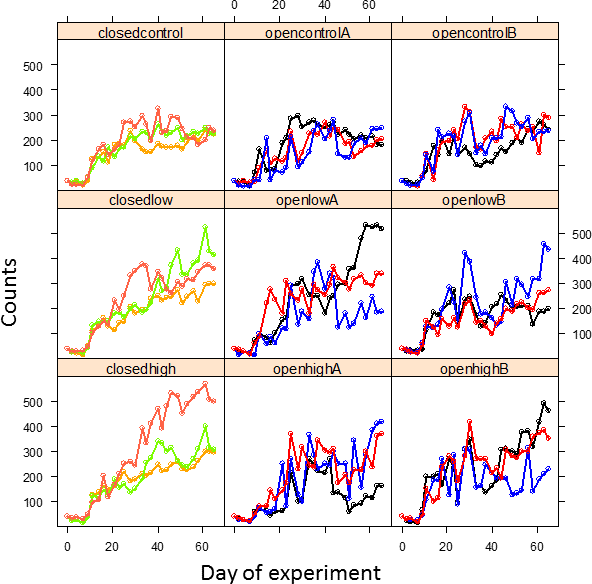
\includegraphics[width=\textwidth]{lectures/day_4_GLS/figures/counts.png}
    \end{column}
\end{columns}
\end{frame}



\begin{frame}{Temporal or Spatial Autocorrelative Structure}
  Allows the residuals of different time or space points to be correlated to each other, following rules given by the specified autocorrelation function.
  \vspace{0.5cm}

  Examplary temporal autorcorrelative functions:
  \begin{itemize}
    \item AR-1 autocorrelation
    \item ARMA autocorrelation
  \end{itemize}
\end{frame}

\begin{frame}{AR-1 Temporal Autocorrelation}
  \[
  \epsilon_t = \rho \cdot \epsilon_{t-1} + \eta_t
  \]
  \[
  \text{cor}(\epsilon_s, \epsilon_t) = 
  \begin{cases}
    1 & \text{if } s = t \\
    \rho^{\vert t-s \vert} & \text{if } s \neq t
  \end{cases}
  \]
  \vspace{1cm}

  \begin{quote}
    \centering
    Decline of relatedness with time.
  \end{quote}
\end{frame}

% \begin{frame}[fragile]{Plotting AR-1 Temporal Autocorrelation}
%   \begin{verbatim}
% par(las = 1, pty = "s", tcl = 0.5, mgp = c(3.5,0.5,0))
% a <- c(1, 0.5, 0.5^2, 0.5^3, 0.5^4, 0.5^5)
% b <- c(1,2,3,4,5,6)
% plot(b, a, type = "n", xlab = "time lag", ylab = "autocorrelation")
% for (i in 1:6){
%   arrows(b[i], 0, b[i], a[i], length = 0, lwd = 3, col = "darkred")
% }
%   \end{verbatim}
%   \begin{center}
%     \includegraphics[width=0.5\textwidth]{ar1_temporal_autocorrelation} % Replace with actual path to plot
%   \end{center}
% \end{frame}

\begin{frame}{AR-1 Correlation Matrix}
\begin{columns}
    \begin{column}{0.5\textwidth}
        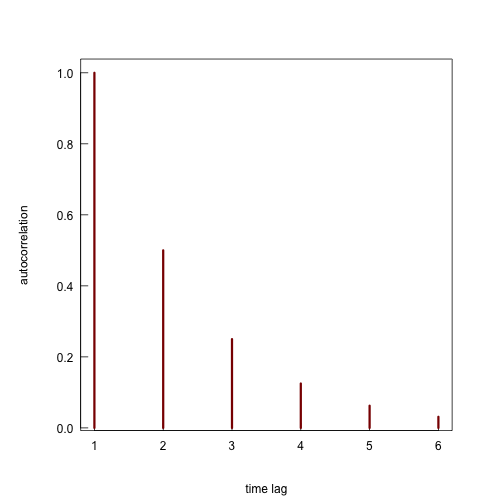
\includegraphics[width=\textwidth]{lectures/day_4_GLS/figures/unnamed-chunk-14-1.png}
    \end{column}
    \begin{column}{0.5\textwidth}
    From the AR-1 structure follows this correlation matrix:
    \[
    \mathbf{V_i} = 
    \begin{bmatrix}
    1 & \rho & \rho^2 & \rho^3 & \rho^4 \\
    \rho & 1 & \rho & \rho^2 & \rho^3 \\
    \rho^2 & \rho & 1 & \rho & \rho^2 \\
    \rho^3 & \rho^2 & \rho & 1 & \rho \\
    \rho^4 & \rho^3 & \rho^2 & \rho & 1
    \end{bmatrix}
    \]    
    \end{column}
\end{columns}

  
\end{frame}

\begin{frame}{ARMA(p,q)-Autocorrelation}
  An AR moving average model where $p$ gives the number of time points before $t$ considered for estimating the correlation of $t$ with the $t - p$ data points. $q$ gives the number of moving average parameters. ARMA(1,0) refers to the AR-1 model.
  
  ARMA(3, 0) gives:
  \[
  \epsilon_t = \phi_1\epsilon_{t-1} + \phi_p\epsilon_{t-2} + \phi_p\epsilon_{t-3}
  \]
  \begin{quote}
    Very flexible as p and/or q increases, but also gets very data-hungry!
  \end{quote}
\end{frame}

\begin{frame}{}
  \begin{columns}
      \begin{column}{0.5\textwidth}
        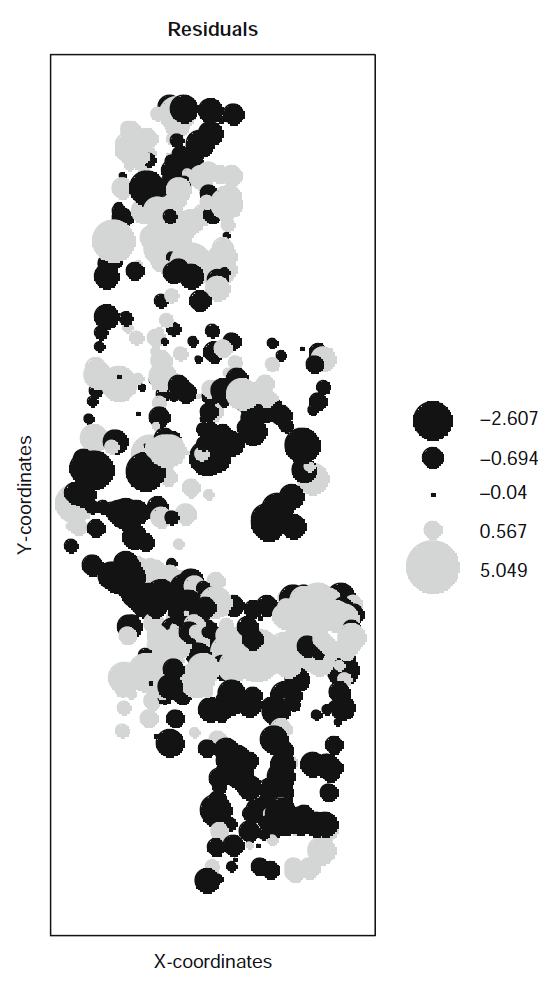
\includegraphics[width=0.9\textwidth]{lectures/day_4_GLS/figures/spatial_residuals.png}
      \end{column}
      \begin{column}{0.5\textwidth}
        \textbf{Spatial Autocorrelations}
        \vspace{0.5cm}
        
        Negative and positive residuals clump together in space.
      \end{column}
  \end{columns}
\end{frame}

\begin{frame}[fragile]
    \frametitle{Shown by a Variogram}
    \begin{columns}
        \begin{column}{0.5\textwidth}
        \centering
        \scriptsize
        \begin{VerbatimIN}[numbers=left,numbersep=6pt]
library(gstat)
        \end{VerbatimIN}
        \vspace{0.5cm}
        
        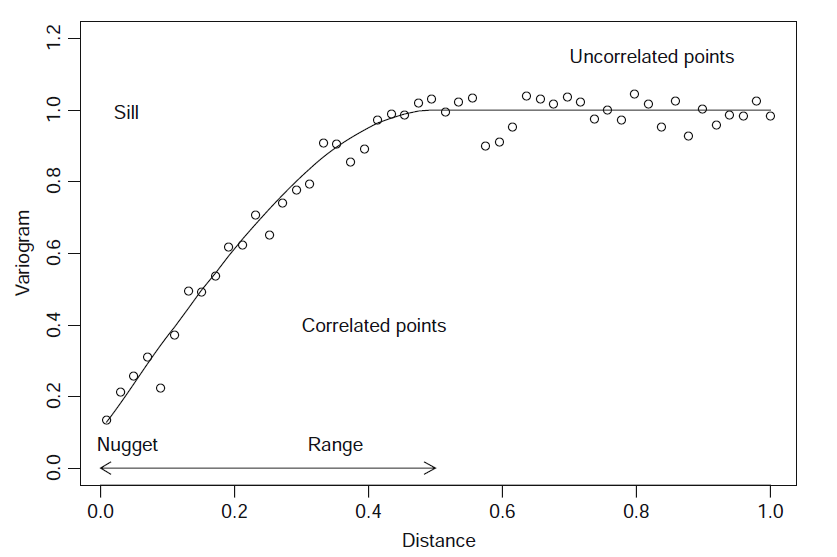
\includegraphics[width=\textwidth]{lectures/day_4_GLS/figures/variogramm.png}
        \end{column}
        \begin{column}{0.5\textwidth}
            Decay of similarity with distance between points.
            \begin{itemize}
                \item The "range" of a variogram is the point at which the curve levels off, i.e., the maximum distance at which data are autocorrelated.
                \item The "sill" is the spatial autocorrelation (SAC) that occurs at a distance equal to the range.
                \end{itemize}
        \end{column}
    \end{columns}
\end{frame}

\begin{frame}{Further Reading}
\centering
  \Large Chapter 7 in: \\
  \textbf{Zuur et al.} \emph{Mixed Effects Models and Extensions in Ecology with R}
  \vspace{0.5cm}
  
  \color{blue}\href{http://highstat.com/index.php/mixed-effects-models-and-extensions-in-ecology-with-r}{here}
\end{frame}

\begin{frame}
  \begin{center}
    \huge\color{purple}\textbf{GLS Examples}
  \end{center}
\end{frame}

\begin{frame}[fragile]{}
\begin{columns}
    \begin{column}{0.4\textwidth}
        \huge\textbf{Example 1: Blowfly Density as a Function of Time}
    \end{column}
    \begin{column}{0.6\textwidth}
        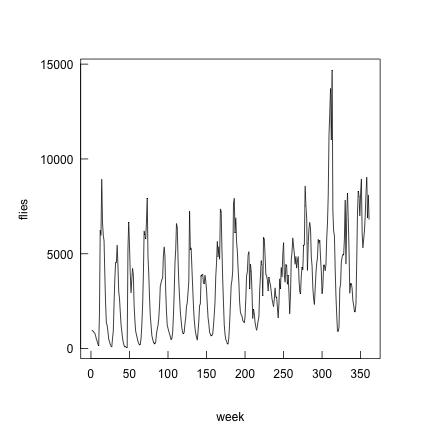
\includegraphics[width=\textwidth]{lectures/day_4_GLS/figures/unnamed-chunk-16-1.png}
    \end{column}
\end{columns}
\end{frame}

\begin{frame}[fragile]
\frametitle{Ignoring Possible Correlation Structure}

\begin{columns}
    \begin{column}{0.63\textwidth}
    \tiny
    \begin{VerbatimIN}[numbers=left,numbersep=6pt]
library(nlme) # contains gls
bf <- gls(flies ~ poly(week,2), na.omit(blowfly))
summary(bf)
    \end{VerbatimIN}
    \begin{VerbatimOUT}[numbers=left,numbersep=6pt]
Generalized least squares fit by REML
  Model: flies ~ poly(week, 2) 
  Data: na.omit(blowfly) 
       AIC      BIC    logLik
  6511.429 6526.951 -3251.715

Coefficients:
                   Value Std.Error  t-value p-value
(Intercept)     3495.956  111.2077 31.43628   0e+00
poly(week, 2)1 21776.334 2112.9459 10.30615   0e+00
poly(week, 2)2  7772.788 2112.9459  3.67865   3e-04

 Correlation: 
               (Intr) p(,2)1
poly(week, 2)1 0            
poly(week, 2)2 0      0     

Standardized residuals:
       Min         Q1        Med         Q3        Max 
-2.1324653 -0.7619228 -0.1771706  0.5515510  4.4766154 

Residual standard error: 2112.946 
Degrees of freedom: 361 total; 358 residual
    \end{VerbatimOUT}  
    \end{column}
    \begin{column}{0.37\textwidth}
        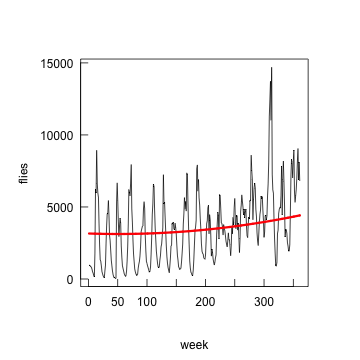
\includegraphics[width=\textwidth]{lectures/day_4_GLS/figures/unnamed-chunk-18-1.png}
    \end{column}
\end{columns}

  
  \begin{center}
    \includegraphics[width=0.5\textwidth]{plot_gls_fitted} % Replace with actual path to plot
  \end{center}
\end{frame}

\begin{frame}[fragile]
\frametitle{Fitting an AR(1) Model}
  \begin{columns}
      \begin{column}{0.7\textwidth}
      \tiny
      \begin{VerbatimIN}
bf.1 <- gls(flies ~ poly(week,2), blowfly, 
correlation = corAR1(form = ~ week))
      \end{VerbatimIN}
      \begin{}
        
      \end{column}
      \begin{column}{0.3\textwidth}
      Using a simple lag-1 autocorrelation model of type AR1 by specifying the \textbf{correlation} argument:
      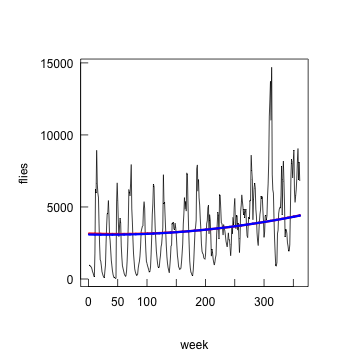
\includegraphics[width=\textwidth]{lectures/day_4_GLS/figures/unnamed-chunk-21-1.png}
      \end{column}
  \end{columns}
\end{frame}

\begin{frame}[fragile]{Auto-Correlation Function (ACF) and Partial ACF}
  A visual detection tool to detect (partial) auto-correlation of residuals.

  \begin{columns}
      \begin{column}{0.5\textwidth}
        \begin{verbatim}
acf(residuals(bf))
        \end{verbatim}
        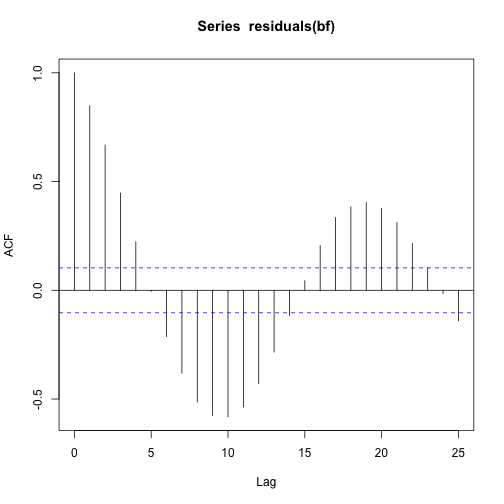
\includegraphics[width=\textwidth]{lectures/day_4_GLS/figures/unnamed-chunk-22-1.png}  
      \end{column}
      \begin{column}{0.5\textwidth}
        \begin{verbatim}
pacf(residuals(bf))
        \end{verbatim}
        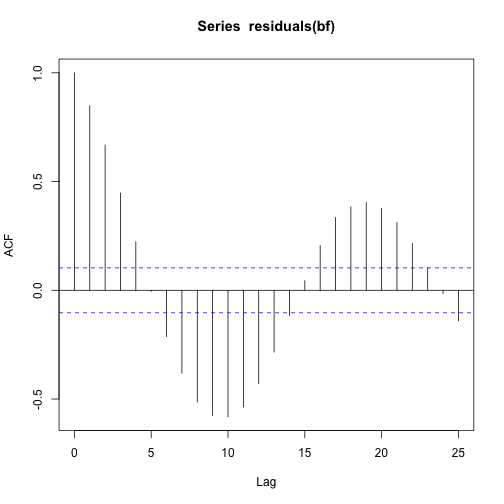
\includegraphics[width=\textwidth]{lectures/day_4_GLS/figures/unnamed-chunk-22-1.png}  
      \end{column}
  \end{columns}
  \tiny Difference between acf and pacf: \color{blue}\href{https://stats.stackexchange.com/questions/483383/difference-between-autocorrelation-and-partial-autocorrelation}{here}
\end{frame}

\begin{frame}[fragile]{Fitting an ARMA(2,2) Model}
  \begin{columns}
      \begin{column}{0.7\textwidth}
      \small
      \begin{verbatim}
bf.2 <- gls(flies ~ poly(week,2), blowfly, 
correlation = corARMA(form = ~ week, p = 2, q = 2))
      \end{verbatim}
      \tiny\scalebox{0.9}{
        \lstinputlisting[]{lectures/day_4_GLS/outputs/output_7.txt}
      }        
      \end{column}
      \begin{column}{0.3\textwidth}
      \newline
      Using a complex moving average autoregressive model of type ARMA(2, 2):
      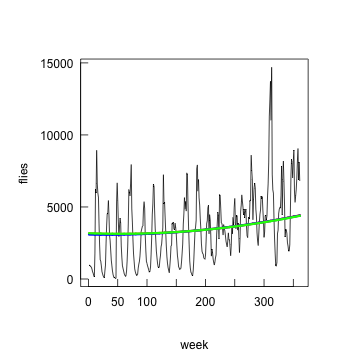
\includegraphics[width=\textwidth]{lectures/day_4_GLS/figures/unnamed-chunk-26-1.png}
      \end{column}
  \end{columns}
\end{frame}

\begin{frame}[fragile]{Model Comparison: Likelihood Ratio Test}
  The fitted models look very similar - is there really a difference? Compare the likelihood ratios.
  \begin{verbatim}
anova(bf, bf.1, bf.2) 
# LRT test says that there is a difference between 
# the AR1 and ARMA(2,2) model
  \end{verbatim}
  \tiny\scalebox{1.2}{
    \lstinputlisting[]{lectures/day_4_GLS/outputs/output_8.txt}
  } 
  \vspace{0.5cm}
  
  \normalsize Yes, there is.
\end{frame}

\begin{frame}[fragile]{ACF and PACF for ARMA(2,2)}
  \begin{columns}
      \begin{column}{0.5\textwidth}
      \begin{verbatim}
acf(residuals(bf.2))
      \end{verbatim}
      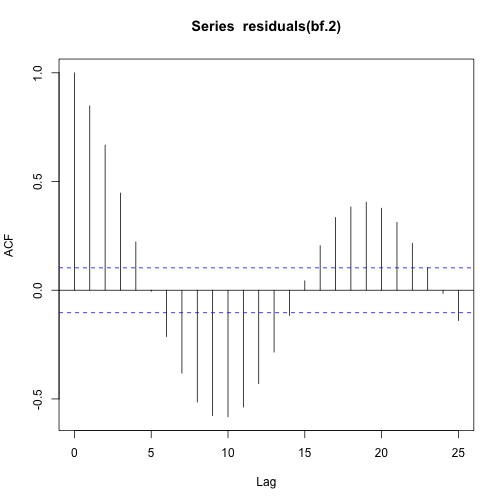
\includegraphics[width=\textwidth]{lectures/day_4_GLS/figures/unnamed-chunk-28-1.png}
      \end{column}
      \begin{column}{0.5\textwidth}
      \begin{verbatim}
pacf(residuals(bf.2))
      \end{verbatim}
      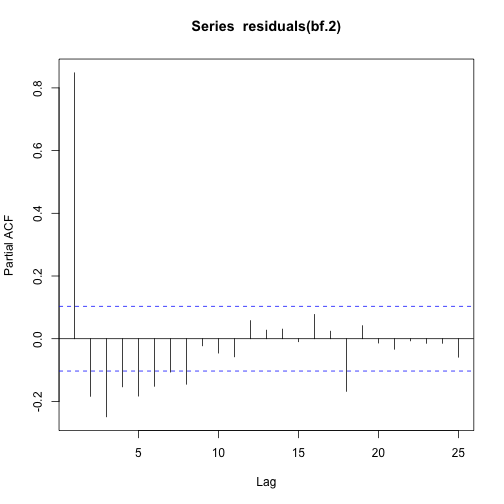
\includegraphics[width=\textwidth]{lectures/day_4_GLS/figures/unnamed-chunk-29-1.png}
      \end{column}
  \end{columns}
\end{frame}

\begin{frame}[fragile]{}
\begin{columns}
    \begin{column}{0.4\textwidth}
        \huge\textbf{Example 2: A Fertilizer Experiment}
    \end{column}
    \begin{column}{0.6\textwidth}
        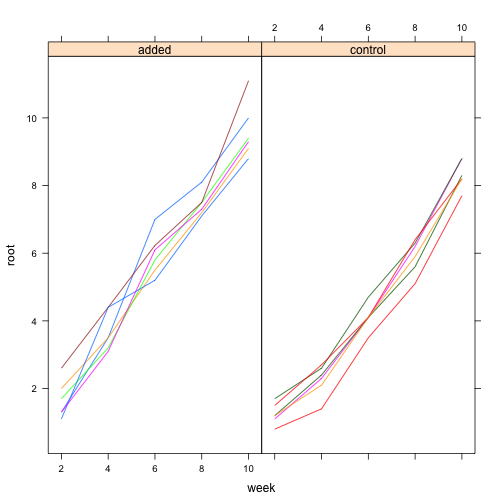
\includegraphics[width=\textwidth]{lectures/day_4_GLS/figures/unnamed-chunk-30-1.png}
    \end{column}
\end{columns}
\end{frame}

\begin{frame}[fragile]{}
\begin{columns}
    \small
    \begin{column}{0.7\textwidth}
      \begin{verbatim}
model.1 <- gls(root ~ week * fertilizer, fertilizer)
summary(model.1)
      \end{verbatim}
    \tiny\scalebox{0.9}{
    \lstinputlisting[]{lectures/day_4_GLS/outputs/output_10.txt}
  } 
    \end{column}
    \begin{column}{0.3\textwidth}
    Again, first without any correlation due to plant:
    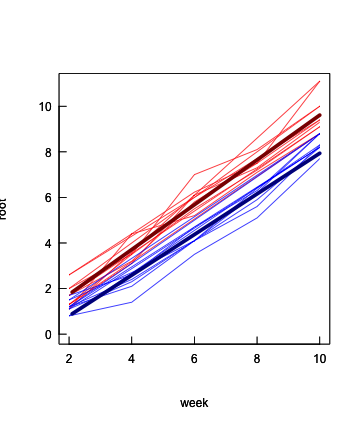
\includegraphics[width=\textwidth]{lectures/day_4_GLS/figures/unnamed-chunk-32-1.png}    
    \end{column}
\end{columns}
\end{frame}

\begin{frame}[fragile]{}
    \begin{columns}
        \begin{column}{0.5\textwidth}
            \begin{verbatim}
acf(residuals(model.1))
            \end{verbatim}
            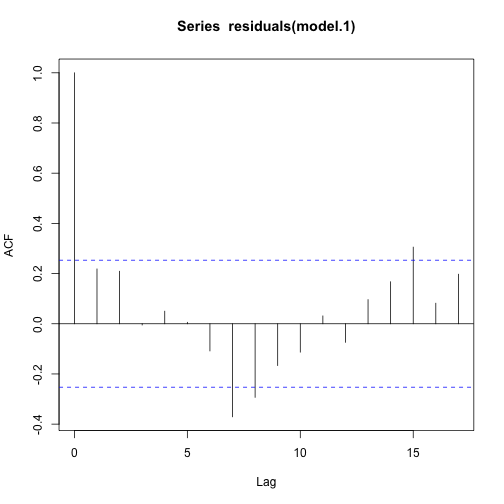
\includegraphics[width=\textwidth]{lectures/day_4_GLS/figures/unnamed-chunk-33-1.png}
        \end{column}
        \begin{column}{0.5\textwidth}
            \begin{verbatim}
pacf(residuals(model.1))
            \end{verbatim}
            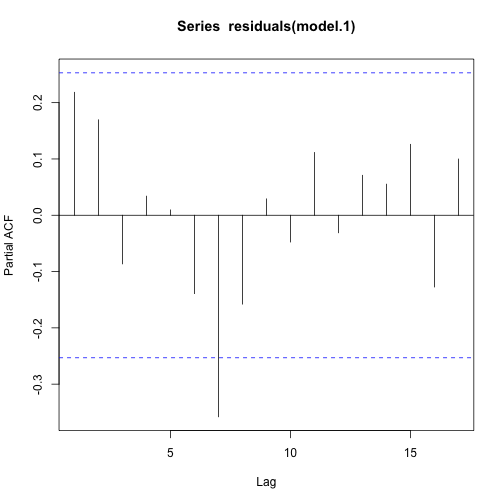
\includegraphics[width=\textwidth]{lectures/day_4_GLS/figures/unnamed-chunk-34-1.png}
        \end{column}
    \end{columns}
\end{frame}

\begin{frame}[fragile]{}
    \textbf{Now testing a compound symmetry correlation due to "plant":}
    \small
    \begin{verbatim}
model.2 <- gls(root ~ week * fertilizer, 
    fertilizer, correlation = corCompSymm(form = ~ week|plant))
summary(model.2)
    \end{verbatim}
    \tiny\scalebox{0.9}{
    \lstinputlisting[]{lectures/day_4_GLS/outputs/output_10.txt}
  } 
\end{frame}

 \begin{frame}[fragile]{}
     \textbf{Any differences?}
     \begin{verbatim}
anova(model.1, model.2)
     \end{verbatim}
     \tiny\scalebox{1.2}{
     \lstinputlisting[]{lectures/day_4_GLS/outputs/output_11.txt}
     } 
     \vspace{0.5cm}
     
     \normalsize\textbf{The variance-covariance matrix of the errors}
     \begin{verbatim}
getVarCov(model1.2)
     \end{verbatim}
     \tiny\scalebox{1.2}{
     \lstinputlisting[]{lectures/day_4_GLS/outputs/output_12.txt}
     } 
     \vspace{0.5cm}
     
     \normalsize\textbf{Get correlation matrix:}
     \begin{verbatim}
cov2cor(getVarCor(model1.2))
     \end{verbatim}
 \end{frame}

\begin{frame}[fragile]{Predictions of the 2nd model}
    \centering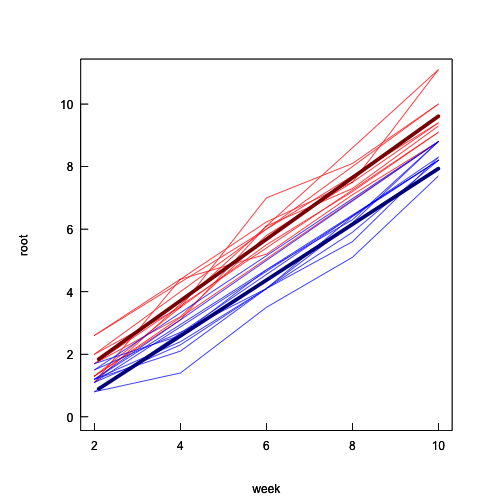
\includegraphics[width=0.7\textwidth]{lectures/day_4_GLS/figures/unnamed-chunk-39-1.png}
\end{frame}

\begin{frame}[fragile]{}
    \begin{columns}
        \begin{column}{0.5\textwidth}
            \begin{verbatim}
acf(residuals(model.2))
            \end{verbatim}
            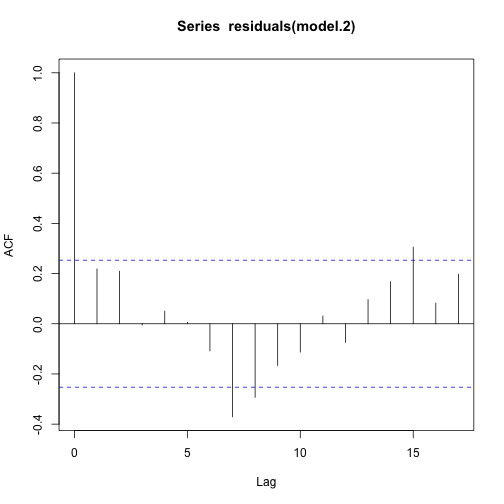
\includegraphics[width=\textwidth]{lectures/day_4_GLS/figures/unnamed-chunk-40-1.png}
        \end{column}
        \begin{column}{0.5\textwidth}
            \begin{verbatim}
pacf(residuals(model.2))
            \end{verbatim}
            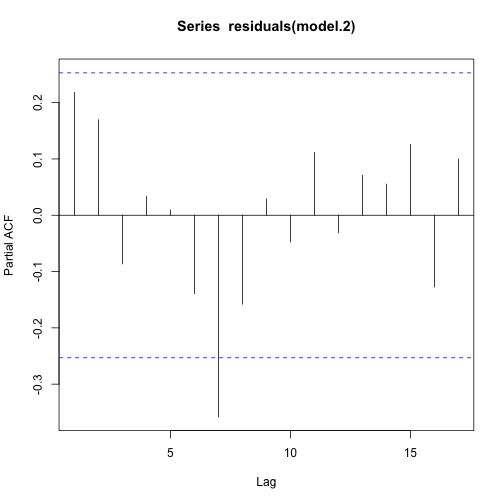
\includegraphics[width=\textwidth]{lectures/day_4_GLS/figures/unnamed-chunk-41-1.png}
        \end{column}
    \end{columns}
\end{frame}

\begin{frame}[fragile]{}
  Use the most complex \textit{general structure} matrix $\mathbf{V_i}$ and look at the correlation part of the output: so many $\rho$ values!
  \tiny
  \begin{verbatim}
model.3 <- gls(root ~ week * fertilizer, 
    fertilizer, correlation = corSymm(form = ~ 1|plant))
  \end{verbatim}
  \tiny\scalebox{0.9}{
     \lstinputlisting[]{lectures/day_4_GLS/outputs/output_13.txt}
     } 
\end{frame}

\begin{frame}[fragile]{}
    \small
    \textbf{The variance-covariance matrix of the errors}
    \begin{verbatim}
getVarCov(model.3)
    \end{verbatim}
    \scalebox{0.7}{
     \lstinputlisting[]{lectures/day_4_GLS/outputs/output_14.txt}
     } 
     \vspace{0.5cm}
     
     \textbf{The correlation matrix of the errors}
     \begin{verbatim}
cov2cor(getVarCov(model.3))
     \end{verbatim}
\end{frame}

\begin{frame}[fragile]{}
    \textbf{Any differences here?}
    \begin{verbatim}
anova(model.1, model.2, model.3)
    \end{verbatim}
    \tiny\scalebox{1.2}{
     \lstinputlisting[]{lectures/day_4_GLS/outputs/output_15.txt}
     } 
\end{frame}

\begin{frame}[fragile]{Some Model Diagnostics}
\small
    \begin{columns}
    \begin{column}{0.5\textwidth}
          \begin{verbatim}
plot(model.3)
          \end{verbatim}
    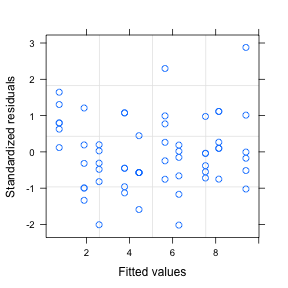
\includegraphics[width=\textwidth]{lectures/day_4_GLS/figures/unnamed-chunk-47-1.png}
    \end{column}
    \begin{column}{0.5\textwidth}
    \begin{verbatim}
qqplot(rnorm(60,0,1), 
as.vector(residuals(model.3)))
    \end{verbatim}
    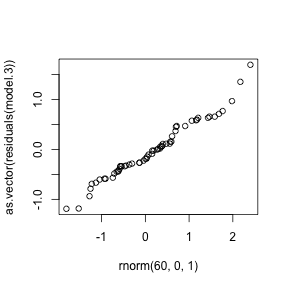
\includegraphics[width=\textwidth]{lectures/day_4_GLS/figures/unnamed-chunk-48-1.png}
         
    \end{column}  
    \end{columns}
\end{frame}

\begin{frame}{Recapitulation Day 4}
  After today you should know and understand:
  \begin{itemize}
    \item How a \textbf{the residual variance-covariance matrix} encodes the assumption of correlation between data points within a group.
    \item What the \textbf{off-diagonals} in a residual covariance matrix are.
    \item The \textbf{assumption} of linear models that is relaxed in GLS.
    \item The difference between \textbf{general}, \textbf{compound symmetric}, and various forms of \textbf{temporal autocorrelation} correlation matrices (AR1, ARMA(p, q)).
  \end{itemize}
  \textbf{Exercises today}: Exercises on GLS. Prepare for tomorrow. Read and discuss paper on Ilias.
\end{frame}

\end{document}
